\section{Methodology}

\subsection{Packet Analysis}
Explain how packets have a specific structure based on the protocol.

\subsubsection{Window Size}
What is Window Size? Where is it stored in the packet? How did we use it to our advantage?

\subsubsection{Time to Live}
What is TTL? Where is it stored in the packet? How did we use it to our advantage?

\subsection{Implementation}
Talk about scapy and python here.
Go through code.

\begin{figure}[p]
	\center{\fbox{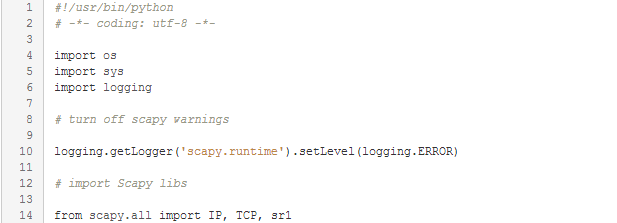
\includegraphics[width=\textwidth]
	{images/code1.png}}}
	\caption{\label{fig:setupCode} Setup Code}
\end{figure}

\begin{figure}[p]
	\center{\fbox{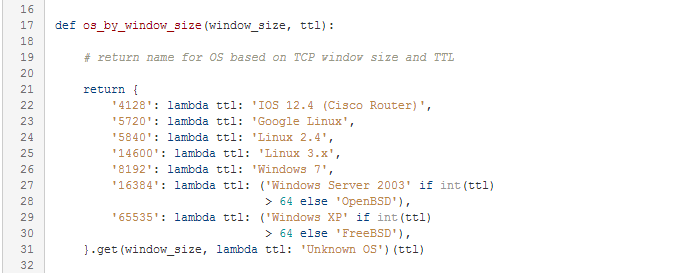
\includegraphics[width=\textwidth]
	{images/code2.png}}}
	\caption{\label{fig:osFunction} OS Identifier Function}
\end{figure}

\begin{figure}[p]
	\center{\fbox{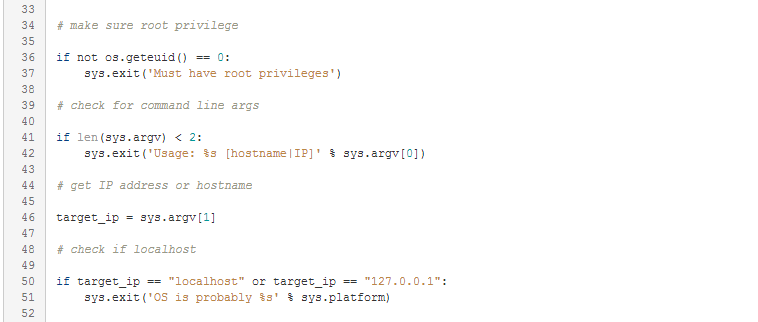
\includegraphics[width=\textwidth]
	{images/code3.png}}}
	\caption{\label{fig:prepare} Input and System Checks}
\end{figure}

\begin{figure}[p]
	\center{\fbox{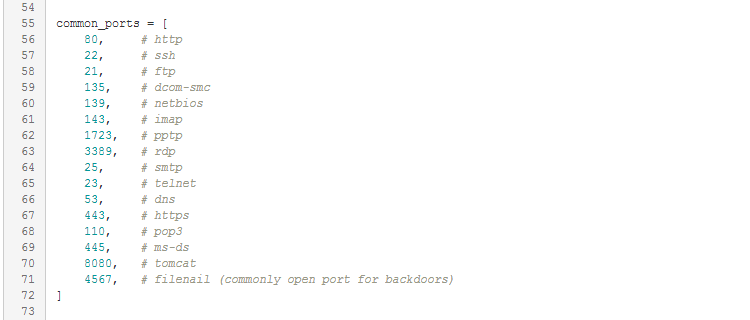
\includegraphics[width=\textwidth]
	{images/code4.png}}}
	\caption{\label{fig:ports} Array of Ports}
\end{figure}

\begin{figure}[p]
	\center{\fbox{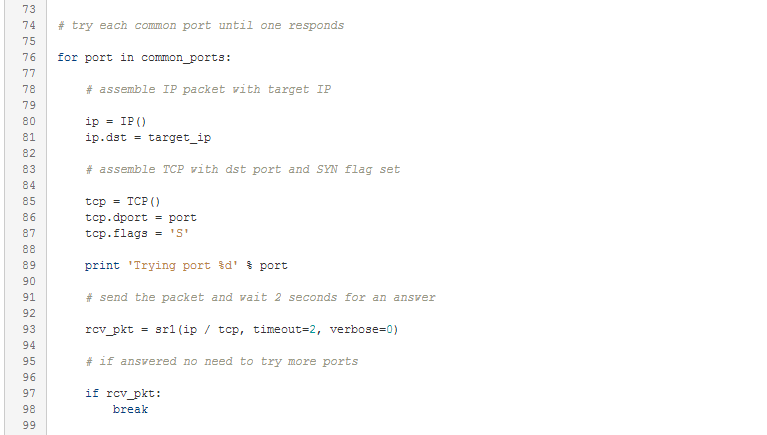
\includegraphics[width=\textwidth]
	{images/code5.png}}}
	\caption{\label{fig:loop} Packet Sending Loop}
\end{figure}

\begin{figure}[p]
	\center{\fbox{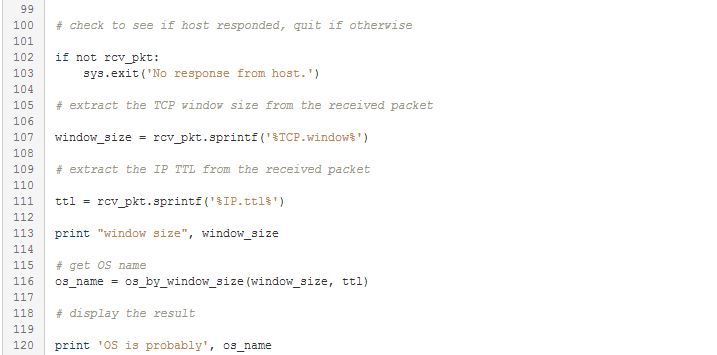
\includegraphics[width=\textwidth]
	{images/code6.png}}}
	\caption{\label{fig:results} Result Interpretation and Output}
\end{figure}

\begin{figure}[p]
	\center{\fbox{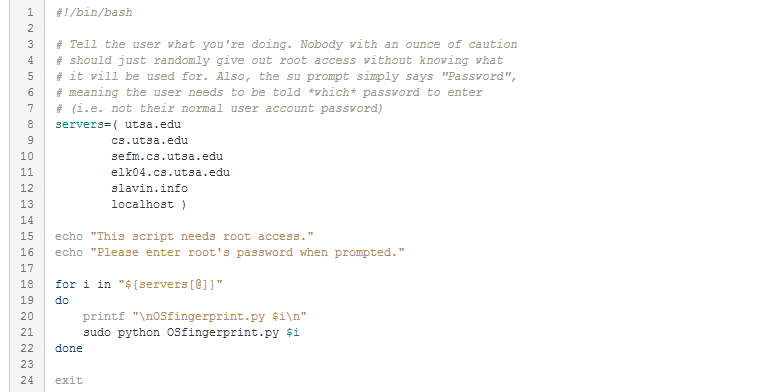
\includegraphics[width=\textwidth]
	{images/testCode.png}}}
	\caption{\label{fig:testScript} Testing Shell Script}
\end{figure}

\subsection{Testing}
Explain how we tested it. Make a long (space taking) table of servers and their OS's

\subsection{Results and Threats}
This might be better as a new section. Not sure if we'd have enough content for it, though.